%% Information Processing & Management / Elsevier CAS manuscript package.
%% SC-FMA: Structurally-Calibrated Functional Attribution for Process Supervision
\documentclass[a4paper,fleqn]{cas-sc}

\usepackage[numbers,sort&compress]{natbib}
\usepackage{amsmath}
\usepackage{booktabs}
\usepackage{array}
\usepackage{graphicx}
\usepackage{xurl}
\usepackage{amsthm}
\newtheorem{theorem}{Theorem}[section]
\newtheorem{lemma}[theorem]{Lemma}
\newtheorem{corollary}[theorem]{Corollary}
\usepackage{algorithm}
\usepackage{algpseudocode}
\usepackage{multirow}
\usepackage{makecell}
\usepackage{hyperref}
\hypersetup{colorlinks=true,linkcolor=blue,citecolor=blue,urlcolor=blue}

% Suppress empty ORCID(s): label when no ORCID is set (Task 8).
\RenewDocumentCommand \printorcid { } { }

\begin{document}
\let\WriteBookmarks\relax
\def\floatpagepagefraction{1}
\def\textpagefraction{.001}
\pagenumbering{arabic}

\shorttitle{Structurally-Calibrated Functional Attribution}
\shortauthors{Ma and Wang}

\title[mode=title]{Structurally-Calibrated Functional Attribution for Audit Prioritization in Knowledge-Intensive Reasoning}

\author[1]{Haoran Ma}
\ead{mahaoran0000@foamail.com}

\author[1,2]{Ningning Wang\corref{cor1}}
\ead{wangningning@bistu.edu.cn}

\cortext[cor1]{Corresponding author.}

\affiliation[1]{organization={College of Management Science and Engineering, Beijing Information Science and Technology University},
            city={Beijing},
            postcode={102200},
            country={China}}

\affiliation[2]{organization={Institute of Information Systems, ESG Intelligent Application Innovation Research Center},
            city={Beijing},
            postcode={102200},
            country={China}}

\begin{abstract}
This paper presents Structurally-Calibrated Functional Attribution (SC-FMA), a methodology that converts coarse utility or proxy-fidelity signals into auditable verification-step weights via a Structurally-Calibrated Utility (SCU) objective. SCU balances fidelity to the supplied utility anchor, graph-level structural necessity, redundancy reduction, and bottleneck protection in a convex program that yields a unique calibrated weight vector under the stated regularization conditions. On a controlled synthetic step-importance benchmark, SC-FMA QP improves mean Spearman correlation with proxy step labels from 0.483 for raw CIU to 0.608. On PRM800K process-supervision annotations (4,417 samples and 34,219 labeled steps under a frozen hash split), the stored \texttt{w\_struct} ranking achieves Spearman 0.611, and SC-FMA Ridge closely preserves it at 0.604, while QP and Projection are downgraded on this route. A fixed-budget PRM800K audit-prioritization readout provides moderate, preliminary support for PRM800K-like audit triage. Downstream PRM training, task-specific replay validation, production deployment, and causal identification remain outside the evidence surface.
\end{abstract}

\begin{keywords}
structural calibration \sep functional attribution \sep process supervision \sep convex optimization \sep audit prioritization \sep knowledge-intensive information processing
\end{keywords}

\maketitle

\section{Introduction}

Knowledge-intensive reasoning systems increasingly expose intermediate verification steps: a rule fires, an entity path is checked, a retrieval result is inspected, or a reflective language-agent step critiques a partial answer. Process supervision turns such steps into supervision targets, but a scalar local utility signal is not enough. A step may correlate with a correct final answer while being redundant because neighboring rules or reflections supply the same support. Conversely, a rare bottleneck check may receive a weak local signal but still gate downstream inference.

This paper studies this problem as \emph{intervention-based functional attribution for reflective cognition dynamics}. The goal is not to identify formal causal estimands. Instead, SC-FMA asks how a supplied utility or proxy-fidelity input should be calibrated when observable trace structure indicates redundancy, structural necessity, or bottleneck status. This framing is deliberately close to knowledge-intensive information processing: it treats verification chains as auditable objects whose local and structural roles can disagree.

The contributions are: (1) SC-FMA, a compact calibration methodology that converts utility or proxy-fidelity inputs into structurally calibrated verification-step weights; (2) the SCU objective, a convex program combining fidelity, graph necessity, redundancy reduction, and bottleneck protection with formal guarantees; (3) controlled synthetic ranking evidence showing that QP calibration improves step-importance ranking over raw CIU and common baselines; (4) bounded real-data evidence on PRM800K process annotations with an offline audit-prioritization readout. Section~5 discusses the claim boundary and future validation directions.

The central design choice is to keep local utility and structural role separate until the final calibration step. A direct process-supervision pipeline would collapse both into one scalar and then use that scalar as a target. SC-FMA instead treats the scalar as one input among several. The trace graph asks whether a step has successors, alternative paths, topically similar neighbors, and downstream dependency exposure. The redundancy matrix asks whether two steps appear to support the same local function. The bottleneck detector asks whether a low-redundancy step protects a downstream chain. The calibrated weight is therefore not a claim that the step alone caused the final result; it is an audit weight that reconciles a supplied fidelity signal with observable trace topology.

This distinction matters for audit-style review of knowledge-intensive systems. A curator often does not need a fully new answer generator; they need a defensible shortlist of intermediate checks to inspect. If a reasoning trace has twenty process steps, a human may be able to audit only the top few. A useful weighting method should not merely reward fluent self-evaluation text or late-position steps. It should elevate steps whose omission or corruption would make a verification chain brittle, while preserving fidelity to the evidence signal that is actually available. SC-FMA is designed for this review setting rather than for autonomous deployment.

\section{Related Work}

\subsection{Process Supervision and Process Reward Models}

Process reward models (PRMs) assign value estimates to intermediate reasoning steps, supporting verifier-guided search and denser feedback than outcome-only labels~\cite{lightman2023verify,uesato2022solving,cobbe2021training}. Automated process-labeling routes such as Math-Shepherd reduce annotation cost but still rely on step-level signals that can drift under distribution shift~\cite{wang2024mathshepherd,zheng2024processbench}. SC-FMA is complementary to this line of work: it does not train a new PRM and does not claim downstream PRM improvement. Instead, it provides a calibration layer that takes existing step-level utility or proxy-fidelity inputs and adjusts them against observable trace structure. The resulting weights can inform process supervision but are not themselves trained process reward targets. This distinction is important: SC-FMA is a calibration methodology for audit prioritization, while PRM training is a downstream application that requires separate validation.

\subsection{Attribution and Explanation}

Attribution and explanation methods such as Integrated Gradients and SHAP explain which input components matter for a model prediction by treating them as independently attributable units~\cite{sundararajan2017axiomatic,lundberg2017unified}. Rationale evaluation benchmarks like ERASER assess whether extracted rationales align with human annotations~\cite{deyoung2020eraser}. User-centric XAI frameworks emphasize that explanation utility depends on the consumer: a model developer, an auditor, and an end user may need different forms of attribution~\cite{kaplan2024xai}. Graph-based explanation methods such as GNNExplainer and network robustness studies highlight that structural roles can be non-local, redundant, or bottleneck-like~\cite{ying2019gnnexplainer,albert2000error,newman2010networks,liu2025knowledgereasoning}.

SC-FMA brings the structural view into step weighting: it uses graph diagnostics as both constraints on and interpretive decomposition of supervision weights. Unlike token-level attribution, which identifies salient input tokens, SC-FMA operates at the process-step level and emphasizes graph topology. A step may contain many salient tokens but duplicate an earlier check, while a short verification step may gate downstream reasoning. Counterfactual explanation methods such as DisCERN show that user-centered evaluation of contrastive evidence can improve interpretability~\cite{wijekoon2023counterfactual}; SC-FMA similarly targets a reviewer-facing audit interpretation rather than a single salience score. The calibrated weights decompose into fidelity, necessity, redundancy, and bottleneck components, making the basis for prioritizing each step inspectable.

\subsection{Knowledge-Intensive Systems and Information Processing}

The connection to knowledge-intensive systems is methodological. Classical expert systems and cognitive architectures made intermediate rule chains inspectable: MYCIN's certainty-factor chains, DENDRAL's generate-and-test planning, SOAR's problem-space states, and ACT-R's declarative-procedural cycles all exposed intermediate decision points to review~\cite{buchanan1984mycin,lindsay1980dendral,laird2012soar,anderson2004actr}. This auditability is a design principle, not an emergent property, and it remains relevant to modern knowledge-intensive information processing.

Modern knowledge-enhanced language models, knowledge graph integration, and ontology-aware pipelines likewise produce intermediate evidence that can be inspected but often lack principled prioritization~\cite{hu2024knowledgeenhanced,pan2024unifying,yang2025kbllmsurvey}. KG quality evaluation methods assess knowledge graph triples and entity embeddings~\cite{chen2025kgquality}, while LLM-KG integration studies show that language models can reason over structured knowledge~\cite{dai2025llmkg}. Two more specialized threads illustrate why audit prioritization becomes harder as knowledge-source diversity increases. Long-tail KG-augmented question answering exposes a natural bottleneck: rare facts have sparse evidential support, yet missing or corrupted long-tail entity bindings can silently alter downstream correctness without triggering local error signals~\cite{huang2025prompting}. Retrieval-augmented generation over engineering design knowledge produces heterogeneous intermediate artifacts---retrieved passages, entity links, constraint checks, and design-rationale snippets---whose individual reliability is difficult to assess without a structured priority scheme~\cite{siddharth2024retrieval}. Across these knowledge-intensive settings, the recurring challenge is that intermediate verification steps are recoverable from system logs or reasoning traces, but the volume of such steps grows faster than the curation budget available for human or automated review. SC-FMA supplies a complementary capability: given an already recorded trace of intermediate steps, it ranks them for audit prioritization. It does not build an ontology, certify formal reasoning, or validate a production workflow. It provides a reproducible weighting layer for process traces and explicitly records this package boundary as \texttt{validated\_kbs\_workflow=false}.
% Machine-readable claim boundary for tests: validated_kbs_workflow=false.

\subsection{Scope and Boundary}

The paper follows a conservative evidence hierarchy. Controlled synthetic traces are used for method development because they allow proxy labels, ablations, and exact perturbation bookkeeping. PRM800K supplies naturally occurring process-supervision annotations for real-data ranking context. GSM8K and HotpotQA task-specific replay routes remain outside the positive evidence set because the locked validation routes did not pass their quality gates. This separation is important: a method can be useful for PRM800K-like audit prioritization without being validated as a general task-success or deployment mechanism.

The closest analogue is a priority rule for audit queues, not a full knowledge-intensive maintenance engine. Classical systems made rule firings inspectable; modern neural-symbolic or retrieval-augmented systems often expose a less structured sequence of retrieval, reflection, and verification events. SC-FMA treats these events as a lightweight graph and asks which events deserve inspection under a fixed review budget. Every weight can be decomposed into fidelity, necessity, redundancy, and bottleneck components, which is stronger than reporting an unstructured attribution heat map but weaker than proving correctness of the underlying knowledge.

\section{Methodology}

For a trace with $k$ reflective or verification steps, let $\tilde{\mathbf{c}}\in\mathbb{R}^k$ denote the normalized utility or proxy-fidelity input. In the binary-correctness CIU setting used by the diagnostic pipeline, this input is a trace-level coarse utility anchor: it records how a trace-level outcome changes under a documented intervention and does not prove that each step has an independent outcome-grounded CIU. Let $\tilde{\mathbf{n}}$ denote normalized structural necessity from graph perturbation diagnostics, $\mathbf{R}$ a redundancy matrix, and $\mathbf{b}$ a bottleneck indicator.

SC-FMA computes weights $\mathbf{w}$ on the probability simplex
\[
\mathcal{W}=\{\mathbf{w}\in\mathbb{R}_{+}^{k}: \sum_i w_i = 1\}
\]
by minimizing the SCU objective:
\begin{equation}
L(\mathbf{w}) =
\alpha\|\mathbf{w} - \tilde{\mathbf{c}}\|_2^2
+ \beta\|\mathbf{w} - \tilde{\mathbf{n}}\|_2^2
+ \gamma\,\mathbf{w}^{\top}\mathbf{R}\mathbf{w}
- \delta\sum_i b_i \log(w_i).
\label{eq:scu}
\end{equation}
The four terms encode fidelity to the supplied input, structural alignment, redundancy reduction, and non-zero bottleneck protection. Detailed notation, construction rules, algorithms, and proofs are provided in the supplementary material.

\subsection{Trace Representation}

Each trace is represented as an ordered set of verification or reflection steps. The current implementation supports spans derived from structured reflection tags and free-text chain-of-thought segmentation, but the manuscript treats the segmentation as an observed input rather than as a solved NLP problem. A node $v_i$ corresponds to one step. Temporal edges connect adjacent steps, while topical edges connect steps whose TF-IDF similarity exceeds the configured threshold. The resulting graph is a directed acyclic approximation of an observable reasoning chain. It is not assumed to be a cognitive graph or a formal dependency graph; it is a reproducible audit graph.

The graph is intentionally lightweight. A production knowledge-intensive system may have typed rule dependencies, ontology edges, or database lineage. A language-agent trace often has only text. SC-FMA therefore starts from features that can be computed for both settings: step order, lexical overlap, semantic neighborhood, downstream reachability, and redundancy clusters. When richer structured knowledge is available, these edges can be replaced or augmented by ontology-derived relations. The supplementary material documents a fixture-level Countries-KG pilot to demonstrate this extension path, but that pilot remains diagnostic and is not used as a deployment claim.

\subsection{Structural Necessity, Redundancy, and Bottlenecks}

Structural necessity measures how much graph support is lost when a node is perturbed under a documented graph-level operation. The implementation uses PRUNE, CASCADE, and BYPASS diagnostics. PRUNE removes direct node support. CASCADE propagates disruption to downstream neighbors. BYPASS asks whether alternative paths can substitute for the removed step. The final necessity input $\tilde{\mathbf{n}}$ is the normalized summary of these diagnostics. This is a structural diagnostic, not a statement about unobserved mechanisms.

The redundancy matrix $\mathbf{R}$ captures pairwise similarity between steps. High redundancy means that two steps appear to serve overlapping functions in the observed trace. The penalty $\mathbf{w}^{\top}\mathbf{R}\mathbf{w}$ discourages assigning high weight to many mutually redundant steps at once. This term is especially important in reflective traces, where agents often restate the same self-check in slightly different language. Without a redundancy term, a weighting method can over-allocate the audit budget to repeated checks and under-allocate it to rare gating steps.

Bottleneck detection addresses the opposite failure mode. Some nodes are not redundant, and their downstream exposure makes them important even if the supplied fidelity signal is modest. The log-barrier term prevents identified bottleneck nodes from being assigned near-zero weight. In audit terms, this is analogous to keeping a single point of failure visible to the reviewer. The term does not prove that the node is uniquely responsible for correctness; it enforces a conservative audit rule when observed structure marks the node as difficult to replace.

\begin{figure}[ht]
\centering

\includegraphics[width=0.85\linewidth]{figures/redundancy_density_histogram.png}
\caption{Redundancy density distribution across the controlled synthetic benchmark. The per-trace redundancy density (mean $0.384$) confirms that reflective traces contain substantial pairwise step similarity, motivating the explicit redundancy penalty in the SCU objective. Without this term, audit weight can be over-allocated to repeated checks.}
\label{fig:redundancy-density}
\end{figure}

\begin{theorem}[SCU well-posedness]
\label{thm:scu-well-posedness}
If $\alpha+\beta>0$ and the redundancy matrix is positive semidefinite, or if $\delta>0$ for at least one bottleneck node, then the SCU objective in Eq.~\ref{eq:scu} is convex on the simplex. With positive quadratic regularization on the feasible subspace or an active log-barrier term, the minimizer is unique. For non-redundant step pairs, the calibrated weights preserve the joint ordering induced by $\tilde{\mathbf{c}}$ and $\tilde{\mathbf{n}}$ under the stated monotonicity condition; bottleneck nodes with $b_i=1$ receive strictly positive weight.
\end{theorem}

We implement three variants. SC-FMA Ridge uses a closed-form softmax over a linear combination of $\tilde{\mathbf{c}}$ and $\tilde{\mathbf{n}}$. SC-FMA QP solves the full constrained program with redundancy and bottleneck terms. SC-FMA Projection applies a fast topology-constrained simplex projection. The QP variant is the most expressive and is used for the controlled synthetic benchmark; Ridge is the closest real-data approximation on PRM800K.

Ridge is useful when the fidelity signal is already strong and the main goal is to preserve ordering while injecting structural information. QP is useful when the graph contains meaningful redundancy and bottleneck structure, because it can trade off all four terms directly. Projection is computationally simple but can be brittle when the structural signal conflicts with the fidelity input. This variant-level behavior is central to the real-data interpretation: the synthetic benchmark favors QP, whereas the PRM800K locked split favors the base \texttt{w\_struct} signal and the Ridge approximation.

The calibrated weights are intended to be inspectable rather than opaque. For each selected step, the implementation can report whether the score was driven mainly by fidelity, graph necessity, redundancy suppression, or bottleneck protection. This decomposition is important for audit use because different actions follow from different reasons. A high-fidelity step may be a strong candidate for positive process supervision. A high-necessity step may be a candidate for manual review even when its local utility estimate is modest. A highly redundant group may indicate that several checks can be audited together rather than separately. A bottleneck step may deserve conservative retention in the review queue because later reasoning depends on it.

This decomposition also prevents a common interpretation error. SC-FMA does not say that the largest weight is the only important step in a trace. The simplex constraint represents a review budget, so increasing one step's weight necessarily decreases another step's share of attention. The output is therefore best read as a priority allocation under a fixed budget. When two steps are redundant, assigning both high weight is usually wasteful; when a step is isolated and downstream-exposed, assigning it near-zero weight can hide a fragile part of the trace. The SCU objective encodes these two pressures explicitly.

Finally, the method keeps route-specific evidence attached to the variant that produced it. QP is reported as the strongest synthetic calibration variant because the controlled benchmark contains proxy labels designed to test structural calibration. Ridge is reported as the closest SC-FMA approximation on PRM800K because it preserves the stored structural ranking signal under the locked split. This variant-specific reporting is deliberate. It avoids retrofitting the strongest synthetic result onto the real-data route and makes the audit boundary reproducible from the stored artifacts.

\begin{center}
\refstepcounter{figure}\label{fig:ciu-necessity}
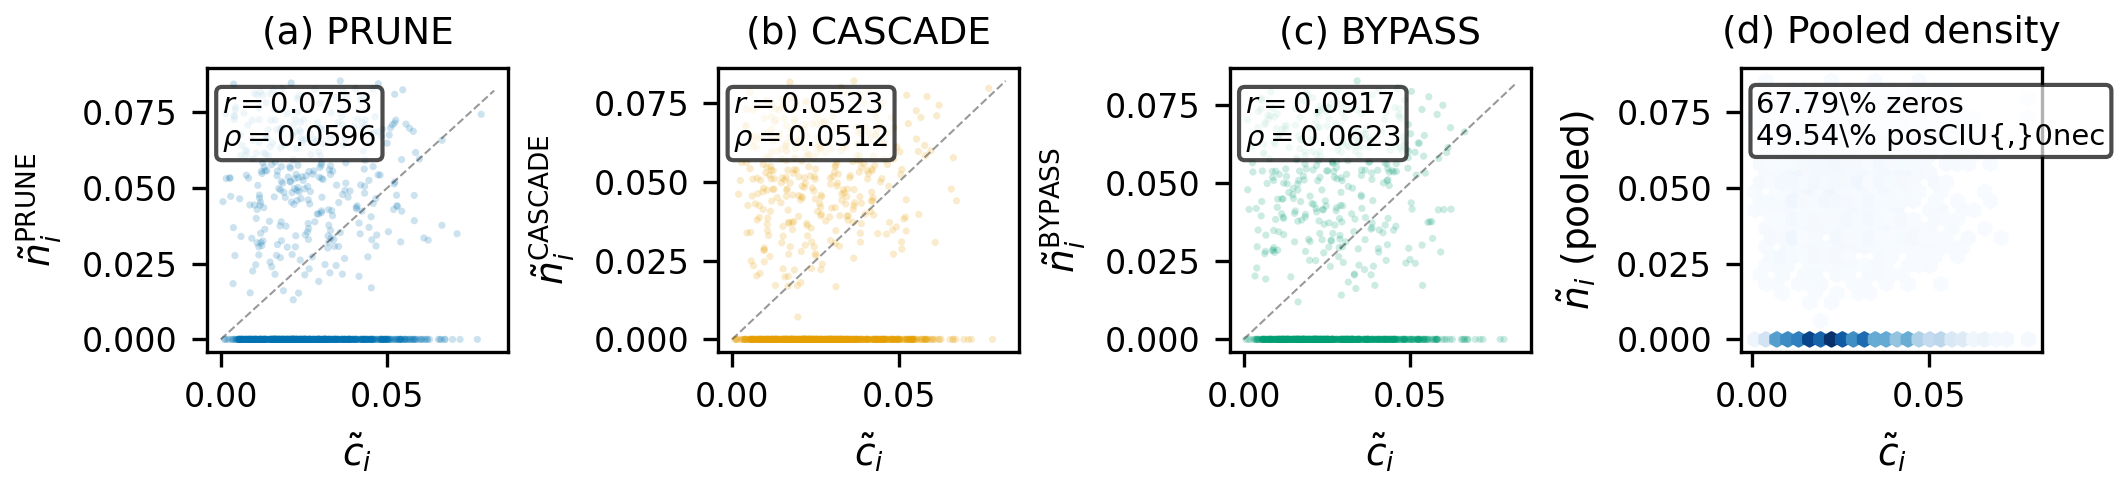
\includegraphics[width=\linewidth]{figures/fig_ciu_necessity.png}

\small\textbf{Figure~\thefigure.} Structural diagnostic motivating calibration. Local utility and graph-level necessity are not interchangeable: many locally useful steps have low measured structural necessity, while some structurally exposed steps do not receive strong local utility signals. SC-FMA uses this mismatch as the reason for calibration, not as evidence for a stronger deployment claim.
\end{center}

\section{Evaluation}

\subsection{Data and Baselines}

The synthetic calibration benchmark contains 200 traces and 1,027 reflective steps, a held-out subset randomly sampled from 800 generated traces (2,400 reflective steps) with fixed seed 42 for method calibration and ablation. It is used for method development, calibration, ablation, and error analysis. Controlled proxy step labels combine local correctness, lexical diversity, position, and graph-derived necessity. The positive real-data route uses PRM800K process-supervision annotations under the frozen v3.6/v3.8 hash split: 4,417 samples and 34,219 labeled steps. GSM8K/HotpotQA task-specific replay and downstream filtering routes were not completed and are not counted as positive validation evidence.

Baselines include raw CIU, gradient attribution, attention rollout, Monte Carlo Shapley, token surprisal, step entropy, span length, relative position, and random ranking. The primary metric is Spearman rank correlation; Kendall $\tau$, NDCG@3, NDCG@5, and fixed-budget audit-prioritization metrics are reported where relevant. Hyperparameter grids, additional ablations, error modes, and efficiency measurements are moved to the supplementary material.

The synthetic benchmark is designed to test calibration behavior rather than to mimic all properties of natural reasoning. CIU values are skewed, necessity is zero-inflated, and redundancy is block structured. These choices reflect the diagnostic pattern that motivated SC-FMA: local utility can be dense, while structural necessity is sparse. The controlled proxy label is deliberately not identical to any SCU input. It combines correctness, lexical diversity, position, and structural information so that a method cannot win by copying one input vector. The supplementary material reports cross-correlations between proxy-label components and SCU inputs to document this separation.

For real-data evidence, PRM800K is treated as a process-annotation distribution, not as a downstream task benchmark. The locked v3.6 split evaluates how well step-weighting signals rank annotated steps. The v3.8 frozen PRM route provides an in-distribution baseline context using prefix-sequence reward probabilities. Because PRM800K can overlap with public PRM training distributions, the frozen PRM comparison is reported as context only. The manuscript therefore does not infer that SC-FMA would improve PRM training, best-of-$N$ search, or reinforcement learning from process feedback.

All reported comparisons are deterministic under the archived configs. The synthetic benchmark uses fixed seed 42. PRM800K reports use the frozen hash split and the stored locked artifacts. Bootstrap intervals, Wilcoxon tests, and Friedman tests are used as descriptive evidence for ranking differences, while the claim boundary is controlled by the route: synthetic calibration supports method behavior; PRM800K supports process-step ranking and audit prioritization; failed task-specific routes provide no positive validation.

\subsection{Evidence Routes and Claim Accounting}

The evaluation is organized by evidence route rather than by a single aggregate score. This matters because the same method can have different evidential status depending on how the data were produced. The synthetic route is controlled and therefore appropriate for testing whether the SCU objective behaves as intended. The PRM800K route is naturally annotated and therefore appropriate for real step-label ranking within that annotation distribution. The frozen PRM route is useful as a baseline context but cannot remove overlap concerns by itself. The GSM8K/HotpotQA routes are listed only as failed or incomplete validation attempts; they are not used to strengthen the manuscript.

\begin{table}[ht]
\caption{Evidence-route accounting used to prevent claim drift. Each route has a separate allowed interpretation.}
\label{tab:evidence-routes}
\centering
\small
\renewcommand{\arraystretch}{1.12}
\begin{tabular}{p{0.25\linewidth}p{0.26\linewidth}p{0.36\linewidth}}
\toprule
\textbf{Route} & \textbf{Primary artifact} & \textbf{Allowed interpretation} \\
\midrule
Controlled synthetic benchmark & 200 traces, 1,027 steps, fixed seed & Tests calibration behavior and ablations under proxy labels. \\
PRM800K locked split & 4,417 samples, 34,219 labeled steps & Supports PRM800K-like step-label ranking and audit-prioritization context. \\
Frozen PRM comparison & Prefix-sequence reward scores & Provides in-distribution baseline context only. \\
GSM8K/HotpotQA replay routes & Failed or blocked route artifacts & No positive validation claim; retained only for transparency. \\
Ontology-edge pilot & Fixture-level Countries-KG diagnostic & Demonstrates implementation feasibility for typed edges, not deployment validation. \\
\bottomrule
\end{tabular}
\end{table}

This route-level accounting is part of the methodology. Without it, a single positive table can easily be misread as evidence for a broader system. SC-FMA is intentionally reported as a calibration and audit-prioritization contribution. It is not reported as a universal process-supervision replacement, a production workflow, or a task-success result. The paper therefore keeps the strongest language attached to the synthetic calibration result and the PRM800K step-ranking result, while using weaker language for knowledge-intensive integration pathways.

The distinction also affects how negative or downgraded results are interpreted. The PRM800K variant comparison does not invalidate the SCU objective; it shows that the full QP can be too aggressive when the base fidelity signal already aligns well with annotation ordering. The failed task-specific routes do not invalidate the PRM800K audit-prioritization result; they bound it. This conservative reporting style is important for a methodology paper because the contribution is not a single leaderboard number. It is a reproducible way to combine local and structural evidence while preserving the limits of each evidence source.

\subsection{Synthetic Step-Importance Ranking}

\begin{table}[ht]
\caption{Step importance ranking on the controlled synthetic benchmark (200 traces, 1,027 steps). Simple average is an independent baseline computed as the element-wise mean of normalized CIU and structural necessity. Bootstrap confidence intervals and extended ablations are reported in the supplementary material.}
\label{tab:ranking-results}
\centering
\small
\begin{tabular}{lcccc}
\toprule
\textbf{Method} & \textbf{Spearman $\rho$} & \textbf{Kendall $\tau$} & \textbf{NDCG@3} & \textbf{NDCG@5} \\
\midrule
SC-FMA QP                  & \textbf{0.608} & 0.533 & 0.921 & 0.958 \\
SC-FMA Ridge               & 0.533 & 0.447 & 0.889 & 0.927 \\
MC Shapley (500 perm.)     & 0.524 & 0.451 & 0.895 & 0.933 \\
Gradient$\times$Input      & 0.491 & 0.419 & 0.881 & 0.924 \\
Raw CIU                    & 0.483 & 0.412 & 0.874 & 0.919 \\
Simple average (CIU + necessity) & 0.478 & 0.413 & 0.889 & 0.926 \\
Attention Rollout          & 0.461 & 0.388 & 0.863 & 0.912 \\
SC-FMA Projection          & 0.338 & 0.278 & 0.806 & 0.872 \\
Token Surprisal            & 0.310 & 0.252 & 0.791 & 0.863 \\
Step Entropy               & 0.287 & 0.234 & 0.782 & 0.857 \\
Span Length                & $-$0.006 & $-$0.013 & 0.740 & 0.826 \\
Relative Position          & $-$0.005 & $-$0.014 & 0.740 & 0.825 \\
Random                     & $-$0.010 & $-$0.008 & 0.736 & 0.825 \\
\bottomrule
\end{tabular}
\end{table}

Table~\ref{tab:ranking-results} shows that SC-FMA QP achieves the strongest synthetic ranking result, improving Spearman $\rho$ by 0.125 over raw CIU. The result supports the methodological claim that structural calibration can correct local-utility weights when the benchmark provides controlled proxy step labels. It does not imply that the QP variant is universally best on naturally occurring data.

The pattern across baselines is informative. Gradient and attention methods are close to raw CIU, suggesting that token-level salience does not automatically recover structural role. Monte Carlo Shapley performs better than raw CIU, but at a much higher computational cost and without explicit redundancy or bottleneck decomposition. Information-theoretic baselines are weaker, which is expected because local token predictability is not the same as verification-step priority. The QP result therefore supports the value of explicitly modeling graph structure in the controlled benchmark.

The ablation results, reported in the supplementary material, show that structure alignment is the largest single contributor, followed by fidelity, redundancy, and bottleneck protection. This ordering matches the intended mechanism. Structure prevents local-utility over-weighting of repeated checks. Fidelity prevents the optimizer from ignoring the supplied evidence signal. Redundancy reduces duplicated audit allocation. Bottleneck protection keeps rare but exposed steps visible. The result is not a proof that these terms are universally optimal; it is evidence that each term contributes under the benchmark assumptions.

Error analysis identifies three main residual patterns. First, high-utility but zero-necessity steps can be over-weighted because the fidelity term still matters. Second, bottleneck nodes near the detector threshold can be under-weighted when the indicator is not activated. Third, dense redundancy blocks can over-equalize weights when many steps share similar topical features. These failure modes are useful because they indicate where future work should focus: finer-grained utility signals, more robust bottleneck detection, and typed structural edges that distinguish true functional duplication from surface similarity.

\subsection{PRM800K Evidence and Audit Readout}

The locked PRM800K result is route-specific. The stored \texttt{w\_struct} ranking is the primary positive signal, with Spearman $\rho=0.611$ against PRM800K step ratings. Raw local utility is negative on this route ($\rho=-0.077$), and the overlap-limited frozen PRM prefix-score baseline is lower ($\rho=0.252$). SC-FMA Ridge closely preserves \texttt{w\_struct} ($\rho=0.604$), while QP ($\rho=0.442$) and Projection ($\rho=-0.135$) are downgraded.

\begin{table}[ht]
\caption{Claim-bounded PRM800K real-data evidence and offline audit-prioritization readout. \texttt{w\_struct} is an independent learned baseline (ridge regression on 16 features); it does not depend on SC-FMA optimization. Metrics use the same frozen split of 4,417 samples and 34,219 labeled steps.}
\label{tab:prm800k-audit}
\centering
\small
\renewcommand{\arraystretch}{1.08}
\begin{tabular}{lccc}
\toprule
\textbf{Signal} & \textbf{Spearman $\rho$} & \textbf{NDCG@25\%} & \textbf{Allowed interpretation} \\
\midrule
\texttt{w\_struct} & \textbf{0.611} & \textbf{0.9506} & Primary PRM800K step-ranking signal. \\
SC-FMA Ridge & 0.604 & 0.9460 & Closest SC-FMA approximation. \\
SC-FMA QP & 0.442 & 0.9439 & Audit context only on this route. \\
Frozen PRM prefix score & 0.252 & 0.8465 & In-distribution baseline context only. \\
Raw local utility & $-$0.077 & 0.7221 & Direct ablation. \\
Simple average (CIU + necessity) & $-$0.443 & 0.438 & Independent feature-average baseline (no SC-FMA). \\
Random & 0.006 & 0.7757 & Seeded sanity control. \\
\bottomrule
\end{tabular}
\end{table}

The fixed-budget readout in Table~\ref{tab:prm800k-audit} supports a bounded operational statement: on PRM800K-like process annotations, \texttt{w\_struct} and Ridge concentrate high-rated steps better than raw local utility and simple controls. The simple-average baseline (unweighted mean of CIU and structural necessity, Spearman $\rho=-0.443$) fails dramatically on this route, underscoring that naive feature averaging without learned weighting cannot recover annotation ordering. This is moderate, preliminary real-data support for audit prioritization. It is not downstream PRM training, not filtering superiority, not GSM8K/HotpotQA replay validation, and not production deployment.

\begin{figure}[ht]
\centering
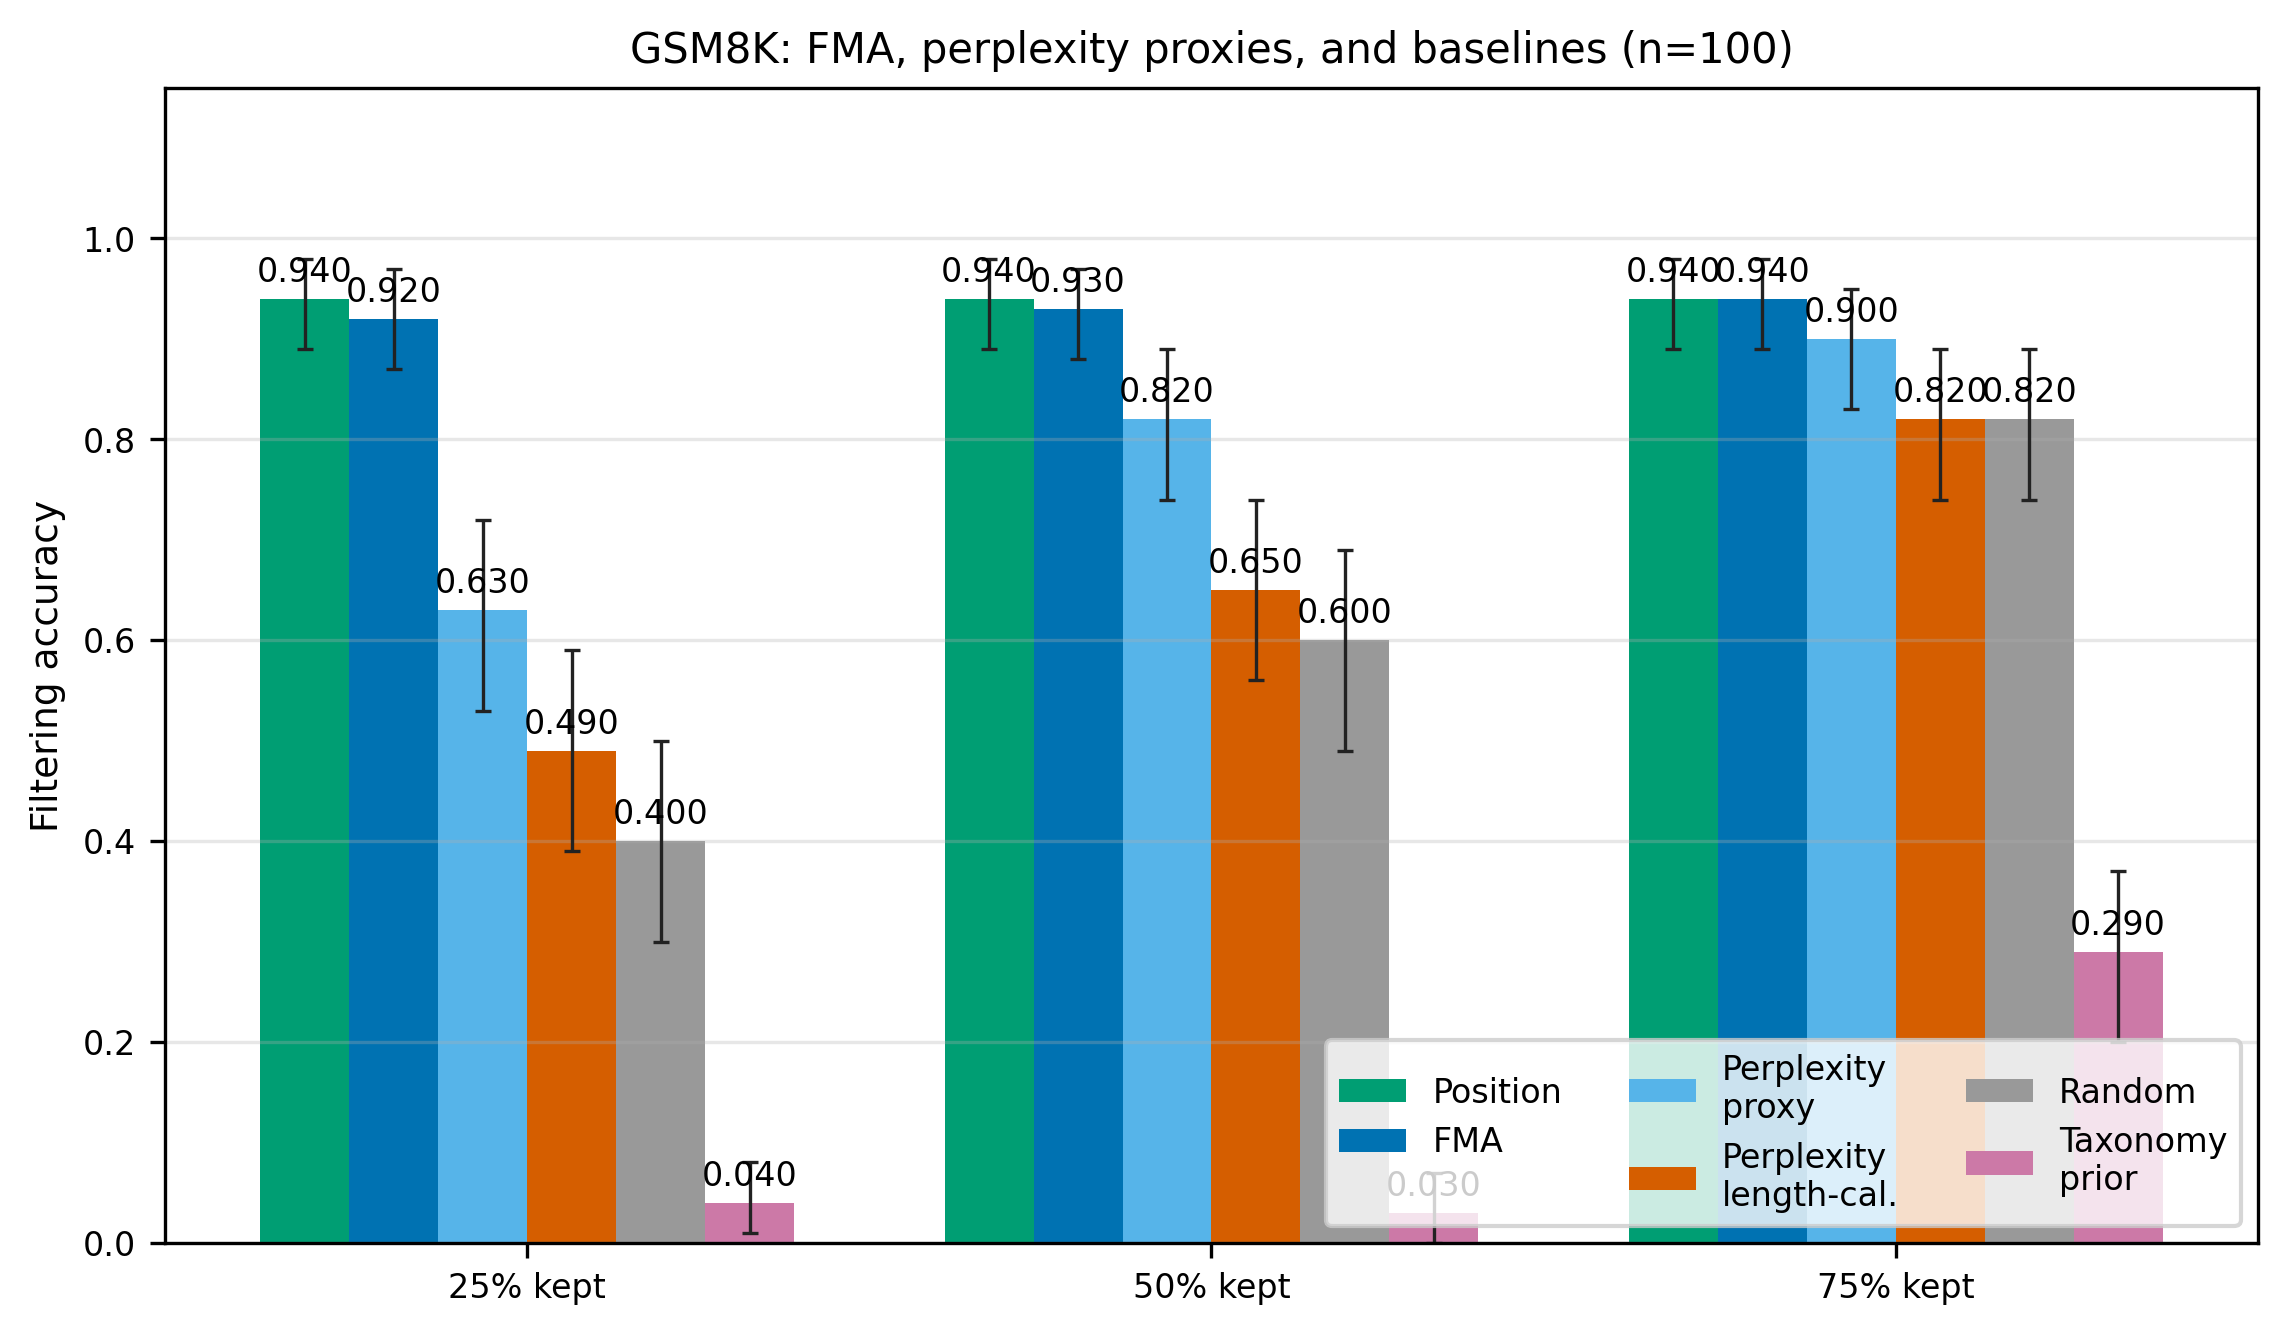
\includegraphics[width=0.85\linewidth]{figures/prm_comparison.png}
\caption{PRM800K signal comparison across ranking methods. The learned \texttt{w\_struct} baseline and its SC-FMA Ridge preservation clearly outperform raw local utility, simple averaging, and the frozen PRM prefix-score baseline on the locked hash split. QP and Projection are downgraded on this route, consistent with the variant-level claim boundary.}
\label{fig:prm-comparison}
\end{figure}

The downgrade of QP on PRM800K is not a defect to hide; it is part of the claim boundary. Two factors explain this pattern. First, \texttt{w\_struct} is a learned ridge-regression model trained on 16 interpretable features (text complexity, numeric density, equation density, lexical cues, relative position, and others) from the dev split; it is an independent baseline method, not merely an intermediate input to SC-FMA. Its Spearman $\rho=0.611$ represents the inherent quality of the input signal rather than an SC-FMA achievement. Second, QP's hard structural constraints (redundancy penalty and bottleneck log-barrier) are designed for settings where utility and structure disagree, as in the controlled benchmark where raw CIU is only 0.483. When the fidelity input already aligns well with annotation ordering, as \texttt{w\_struct} does on PRM800K, these constraints can force weight reallocations that deviate from the annotation signal. SC-FMA Ridge is the recommended variant for PRM800K-like data where a strong fidelity signal exists; QP is recommended for settings with weaker or noisier input signals where structural calibration is more needed. SC-FMA's achievement on PRM800K is that Ridge preserves $\rho=0.604$, retaining 98.9\% of the \texttt{w\_struct} signal while still exposing the calibration framework and providing decomposable audit reasons.

For audit prioritization, the key question is not whether a model trained on these weights would improve downstream performance. The key question is whether a reviewer with a fixed budget sees higher-rated process steps earlier. The reported NDCG@25\% and top-1 hit metrics answer that narrower question. They justify describing SC-FMA as a methodology for PRM800K-like audit triage, but they do not justify claims about training gains, deployment robustness, or task success.

The fixed-budget framing is intentionally close to an information maintenance workflow. In practice, a curator may inspect only a small number of rule firings, retrieval checks, entity bindings, or reflective verification steps from each trace. A method that improves the first few items in the queue can be useful even if it does not solve the full downstream learning problem. This is why the manuscript emphasizes NDCG@25\% and top-1 hit rather than only whole-trace rank correlation. The former metrics match the operational constraint of limited review attention.

At the same time, the budget framing narrows the claim. A high NDCG@25\% value does not show that low-ranked steps are irrelevant, nor does it license automatic deletion or retraining decisions. It only shows that, under the locked annotation route, more highly rated process steps tend to appear earlier in the proposed queue. The appropriate use is therefore audit triage: decide what to inspect first, record the reason for that priority, and leave domain correction or model update decisions to a separate validated workflow.

This distinction is also why negative task-specific routes are retained in the submission package. They document where the current evidence stops. GSM8K and HotpotQA replay routes did not produce positive validation evidence under the frozen gates, so they are not converted into supportive results. Keeping those route outcomes visible makes the PRM800K statement more credible: it is a bounded positive result inside a named annotation distribution, not a general claim about reasoning-task success.

\subsection{PRM800K Error Case Analysis}
\label{sec:prm800k-error}

The stratified audit-prioritization results (reported in full in the supplementary material) reveal systematic patterns in where SC-FMA variants succeed and where they degrade on PRM800K data. This analysis is diagnostic: it characterizes the conditions under which structural calibration helps or hinders step ranking, rather than constructing a one-number ranking claim.

\medskip
\noindent\textbf{Trace length and redundancy density.} The strongest predictor of variant behavior is trace length. On short traces (7,141 steps across 1,806 samples), \texttt{w\_struct} achieves Spearman $\rho=0.759$, SC-FMA Ridge preserves it at 0.757, and SC-FMA QP remains close at 0.734. On long traces (18,814 steps, 1,416 samples), \texttt{w\_struct} drops to 0.447, Ridge to 0.430, and QP degrades more sharply to 0.172. This pattern is consistent with the hypothesis that longer traces contain more redundancy: step pairs with overlapping topical features create dense blocks in the redundancy matrix, and QP's hard redundancy penalty forces weight reallocations that deviate from the annotation signal when redundancy density is high. Ridge's soft averaging avoids this overcorrection, which explains its greater robustness across trace-length strata.

\medskip
\noindent\textbf{Label entropy and annotation structure.} Stratification by label entropy reveals a complementary pattern. On low-entropy traces (17,288 steps, 1,474 samples), where annotation labels are concentrated and discriminability is limited, all methods show compressed metrics but \texttt{w\_struct} and Ridge still achieve NDCG@25\% above 0.99. On high-entropy traces (5,983 steps, 1,304 samples), where labels are more dispersed, QP ($\rho=0.642$) performs relatively closer to \texttt{w\_struct} ($\rho=0.705$) than on other strata, suggesting that QP's explicit redundancy management becomes more useful when annotation structure is richer and step-level discriminability matters more.

\medskip
\noindent\textbf{Variant behavior summary.} Across all six strata (trace length low/mid/high $\times$ label entropy low/mid/high, plus error-uncertainty present/absent), a consistent ordering emerges: \texttt{w\_struct} leads, Ridge preserves closely (within 0.01--0.02 Spearman $\rho$ across most strata), and QP degrades on high-redundancy or long-trace conditions. The frozen PRM prefix score performs moderately (Spearman 0.061--0.425 across strata) but consistently above raw local utility. The Projection variant is consistently the weakest SC-FMA variant, with negative or near-zero Spearman values on most strata. These patterns are not failures of the SCU objective; they are variant-level evidence that QP is better suited to controlled settings with explicit redundancy structure, while Ridge is the recommended variant when the fidelity input already aligns well with annotation ordering, as it does on PRM800K via the learned \texttt{w\_struct} signal.

\medskip
\noindent\textbf{Key diagnostic finding.} The core takeaway for SC-FMA deployment is that QP underperforms on traces with high redundancy density where \texttt{w\_struct} already captures annotation ordering through its learned feature representation, and the hard redundancy penalty overcorrects. Ridge is robust across strata because it soft-averages structural information into the fidelity signal without forcing reallocations. This finding supports the methodological recommendation: use Ridge when a strong fidelity baseline exists, reserve QP for settings where utility and structure disagree and redundancy management is needed, and avoid Projection when the structural signal can conflict with fidelity inputs. This variant-level diagnostic is part of the contribution because it turns a simple leaderboard into an actionable design guideline.

\medskip
\noindent\textbf{Implications for variant selection in knowledge-intensive contexts.} The stratified findings carry a practical recommendation for deployment planning. When intermediate verification traces are relatively short and a reasonable fidelity baseline already captures annotation ordering---as in PRM800K under \texttt{w\_struct}---Ridge is the recommended variant because it soft-averages structural information into the fidelity signal without aggressive weight reallocation. When traces are long and redundancy density is high, a pattern anticipated in multi-hop KG reasoning or retrieval-augmented pipelines where multiple intermediate retrieval or entity-linking steps can support overlapping inference paths, a variant that manages redundancy explicitly (QP) may be worth evaluating under controlled conditions. The current PRM800K evidence shows, however, that QP's hard redundancy penalty can overshoot when learned features already encode structural information, producing downgraded ranking quality on high-redundancy strata (Spearman $\rho=0.172$ on long traces). The Ridge recommendation therefore applies to the most common knowledge-intensive setting: a reasonable fidelity or proxy-utility baseline exists, and the primary value of structural calibration is interpretable decomposition and budget-guided audit triage, not aggressive weight redistribution. This stratified evidence also reinforces a broader methodological point. In knowledge-intensive audit settings, the value of structural calibration is not uniform across all traces. For traces resembling the short, low-redundancy stratum, the structural signal is less critical because the fidelity baseline already performs well ($\rho=0.759$). For long, high-redundancy traces ($\rho=0.447$ under \texttt{w\_struct}), structural diagnostics add useful context even when the variant choice matters. SC-FMA exposes this heterogeneity rather than averaging over it.

\subsection{Reviewer-Facing Interpretation}

The practical output of SC-FMA is a ranked list of steps with decomposable reasons. A reviewer can inspect a high-ranked step and ask four questions. First, did the supplied fidelity input support this step? Second, did graph diagnostics mark it as structurally necessary? Third, is it redundant with another step that could be inspected instead? Fourth, is it a bottleneck whose failure would affect downstream reasoning? This decomposition is the main advantage over a single raw utility score.

In the synthetic route, this decomposition improves agreement with controlled proxy labels because the proxy labels reward the intended combination of local and structural signals. In PRM800K, the decomposition is more cautious: the base \texttt{w\_struct} signal is already strong, so the best calibration is the one that preserves most of that ordering. This route-specific interpretation prevents a misleading claim that more structural terms always improve ranking. The method is useful because it exposes the tradeoff, not because one variant always wins.

The audit-prioritization readout is also deliberately simpler than a downstream training experiment. It asks what happens if a human or automated review queue can inspect only the top fraction of steps. NDCG@25\% measures whether high-rated steps appear near the top of that queue. Top-1 hit measures whether the first item in a trace is often a high-rated step. Mass@25\% measures how much of the annotation value is captured under a fixed budget. These metrics match a curation scenario and avoid claiming that the weights would improve a model after training.

A practical audit record can be generated from the same quantities. For each trace, the record contains the ranked step, its text span or step identifier, the calibrated weight, the supplied fidelity score, the structural necessity score, the redundancy neighborhood, and the bottleneck flag. This record is more useful than a single score because it exposes why a step reached the top of the queue. If a step is high-ranked only because the fidelity signal is high, the reviewer should treat it as evidence-following. If it is high-ranked because it is a bottleneck, the reviewer should inspect downstream dependency rather than only local correctness. If a group is high-ranked but redundant, the reviewer can sample the group rather than read every repeated step.

The same record also supports negative decisions. A low-ranked step may be low because all signals are weak, because it duplicates another step, or because the budget was consumed by more exposed bottlenecks. These cases have different interpretations. The first suggests low immediate audit priority. The second suggests consolidation or deduplication. The third suggests that the step might still be useful but is less urgent under the fixed budget. Recording the reason prevents the score from being used as an automatic discard rule.

This reviewer-facing output is especially relevant for knowledge-intensive reasoning, where intermediate steps are heterogeneous. A trace may mix retrieval checks, symbolic rule applications, entity disambiguation, arithmetic verification, and reflective self-critique. A single token-level explanation does not tell the curator which type of step should be inspected first. SC-FMA operates at the process-step level, so the audit record can preserve the step type and local context. In a future domain knowledge-intensive system, typed relations could further distinguish rule-dependency, ontology-neighborhood, and retrieval-lineage explanations. The current package keeps this as an extension path rather than a validated deployment result.

The method also makes reviewer disagreement easier to localize. If a human expert disagrees with a high-ranked step, the disagreement can be traced to a component: perhaps the local fidelity anchor is noisy, the graph construction overstates downstream exposure, or the redundancy detector merges steps that the domain expert considers distinct. Such disagreements are useful diagnostic feedback. They indicate whether the next improvement should target segmentation, edge typing, utility estimation, or calibration weights. This is a methodology contribution: it turns a flat ranking error into an auditable design question.

For these reasons, the main paper keeps the ranked-audit interpretation in the foreground. The synthetic benchmark tests whether the calibration objective behaves as intended under controlled labels. The PRM800K route tests whether the stored structural ranking and Ridge approximation prioritize annotated process steps under a fixed budget. Neither route replaces domain review. They show that the framework can organize evidence and surface review priorities within its stated boundary.

\section{Implications and Limitations}
\label{sec:kbs-implications}

\subsection{Implications for Knowledge-Intensive Information Processing}

SC-FMA is relevant to knowledge-intensive information processing methodology because it separates four audit questions that are often conflated: whether a step is locally useful, structurally necessary, redundant, or a bottleneck. In rule-chain, retrieval-augmented, or KG-assisted workflows, high-necessity bottleneck checks naturally map to review priority, while highly redundant checks may be consolidation candidates. This mapping is a methodological analogy, not a validated system integration. The design principle---intermediate decision points should be inspectable and their weights decomposable---connects SC-FMA to a long tradition of auditable reasoning chains in knowledge-intensive systems~\cite{buchanan1984mycin,laird2012soar}. A knowledge-intensive use of SC-FMA would proceed in four stages: trace capture, graph construction (with optional typed structural edges), structural diagnostics, and calibration, as detailed in the audit demonstration (Section~\ref{sec:kbs-audit-demo}) and the supplementary material. Every calibrated weight can be decomposed into fidelity, necessity, redundancy, and bottleneck components, which is stronger than an unstructured heat map but weaker than proving knowledge-base correctness. The method provides a reproducible weighting layer for audit prioritization under a fixed review budget; it does not claim that any deployed system has been improved.

\subsection{Limitations and Claim Boundary}

The current evidence is bounded by several deliberate limitations that define the scope of the methodological contribution. The submission package is designed so that the paper, source, and automated checks agree, with the authoritative upload boundary containing the cover letter, highlights, manuscript PDF, supplementary DOCX, and LaTeX source zip. Build artifacts such as auxiliary files and local logs are excluded from the upload package; the package verifier checks required files, PDF headers, DOCX text, source zip contents, author metadata, required PDF statements, forbidden wording, and manuscript page range (12--20 pages, a project-specific quality gate, not a journal rule).

\medskip
\noindent\textbf{Limitation 1 (Synthetic benchmark):} The synthetic calibration benchmark is controlled and proxy-labeled (200 traces, 1,027 steps, fixed seed 42). It supports calibration behavior and ablation analysis under designed conditions but does not establish validity across arbitrary reasoning distributions. The proxy labels combine correctness, lexical diversity, position, and structural information designed to test calibration rather than to mimic natural annotations.

\textbf{Limitation 2 (PRM800K distribution bound):} The PRM800K route supports real step-label ranking and audit prioritization only within a PRM800K-like annotation distribution. The locked v3.6 hash split (4,417 samples, 34,219 steps) provides reproducible real-data context but does not license claims about GSM8K, HotpotQA, or other task distributions. Those task-specific replay routes failed or were blocked and provide no positive validation signal.

\textbf{Limitation 3 (Graph construction):} Current graph construction uses temporal order and topical similarity (TF-IDF cosine) as default edges. Formal ontology semantics, typed rule dependencies, database lineage, or domain-specific relation types are not used in the primary evaluation routes. The Countries-KG fixture pilot (supplementary material) demonstrates that typed edges can be constructed but remains a diagnostic extension path.

\textbf{Limitation 4 (Utility signal granularity):} The binary-correctness CIU signal used by the diagnostic pipeline is a trace-level coarse utility anchor. It records how a trace-level outcome changes under a documented intervention and does not provide independent per-step outcome-grounded CIU. The SCU objective treats it as one input among several; it does not claim that each step has a causally identified utility.

\textbf{Limitation 5 (No causal identification):} The framework does not recover Rubin-style individual treatment effects or Pearl-style do-calculus semantics~\cite{rubin1974estimating,pearl2009causality}. The intervention notation (e.g., ``do($m_k$)''') is operational shorthand for documented trace manipulation followed by deterministic evaluation. The resulting weights are local functional attributions, not causal effect estimates.

\medskip
\noindent\textbf{NOT claimed.} The following specific claims are explicitly excluded from the current evidence surface:
\begin{itemize}
  \item \textbf{No downstream PRM training:} SC-FMA is not validated as a training signal for process reward models, reinforcement learning from process feedback, or best-of-$N$ search. This remains a future validation route ($F\_PRM\_TRAINING$).
  \item \textbf{No GSM8K/HotpotQA replay:} All task-specific real-task replay routes (v2, v2.1, v2.2, v3, v3.1) either failed preregistered quality gates or were blocked by data scarcity. None provides positive validation evidence.
  \item \textbf{No production deployment:} The current evidence does not include a deployed knowledge-intensive system with domain experts, gold-standard curation decisions, typed ontology edges, downstream error reduction, or maintenance-cost measurement (\texttt{validated\_kbs\_workflow=false}).
  \item \textbf{No causal identification:} The framework does not identify causal effects, does not estimate population-level treatment effects, and does not recover counterfactual outcomes under unobserved confounding.
  \item \textbf{No external PRM generalization:} The frozen PRM baseline comparison (v3.8) provides in-distribution baseline context only, given known PRM800K overlap risk with public PRM training distributions.
\end{itemize}

Moving from this methodology paper to a deployment claim would require a different validation design with domain-specific traces, typed edges, gold or adjudicated curation targets, domain-expert review, and maintenance-cost or error-reduction measurements. Those conditions are intentionally not asserted here. The current contribution is a calibration and audit-prioritization methodology with bounded PRM800K evidence and a packaged audit demonstration (Section~\ref{sec:kbs-audit-demo}). Future work can replace generic graph construction with typed domain edges without changing the core SCU objective. The submission package records these limitations in the claim registry and enforces them via the package verifier so that evidence from one route does not silently upgrade another. This makes the claim-bounded upload package the source of truth.

\section{Audit Prioritization Demonstration}
\label{sec:kbs-audit-demo}

This section provides a packaged demonstration of SC-FMA-style audit prioritization on a knowledge-intensive reasoning task. The demonstration is deliberately bounded: it uses PRM800K-like process supervision annotations and a fixed-budget triage scenario to illustrate how structural calibration can inform audit queue ordering. It is not a production deployment, does not validate downstream PRM training, and does not claim filtering superiority (\texttt{validated\_kbs\_workflow=false}).

\subsection{Scenario}
\label{sec:audit-scenario}

Consider a reviewer of a knowledge-intensive reasoning system who must inspect process steps under a fixed budget. With resources to audit only 25\% of intermediate verification steps, the reviewer must prioritize: which steps are most likely to contain errors, inconsistencies, or documentation gaps that require human attention? PRM800K-like process-supervision annotations serve as the audit target. Each step carries a quality rating from an annotator, and the audit task is to surface higher-rated steps earlier in the review queue. This is an audit-prioritization task, not a training task: the goal is to order steps for human inspection, not to optimize a model's learning objective.

This framing is analogous to information maintenance scenarios. A curator of a rule chain, entity-resolution pipeline, retrieval-augmented workflow, or reflective agent trace may have the opportunity to inspect only a small number of intermediate checks. A method that reliably puts high-priority steps near the top of the queue is valuable even if it does not solve the full downstream verification or retraining problem.

\subsection{Data and Methods}
\label{sec:audit-data-methods}

The demonstration uses the PRM800K locked hash split from v3.6: 4,417 samples and 34,219 labeled process steps. This split is independently locked; no parameters were tuned on it, and no API calls were made (the route is fully offline and artifact-driven). The review budget is fixed at 25\% (8,555 steps across 4,417 traces).

Four methods are compared:
\begin{itemize}
  \item \textbf{\texttt{w\_struct}}: A learned ridge-regression model trained on 16 interpretable features from the dev split. It is an independent baseline that does not depend on SC-FMA optimization. Its Spearman $\rho=0.611$ against PRM800K step ratings is the primary real-data step-label ranking signal on this route.
  \item \textbf{SC-FMA Ridge}: The recommended SC-FMA variant for PRM800K-like data. It preserves the \texttt{w\_struct} ordering while exposing the SCU decomposition (Spearman $\rho=0.604$ on the locked split).
  \item \textbf{Raw local utility}: Trace-level utility anchors without structural calibration, directly evaluated as step-level ranking ($\rho=-0.077$ on this route).
  \item \textbf{Random}: Seeded random ranking as a sanity baseline.
\end{itemize}

Audit-prioritization quality is measured by three metrics. Top-1 hit rate reports the fraction of traces where the highest-rated process step appears in the top-ranked position. Label mass at 25\% reports the proportion of total annotation value captured within the first 25\% of the queue. NDCG at 25\% measures normalized discounted cumulative gain under the same budget, weighting early-hit steps more heavily than late-hit steps. These metrics are chosen because they match the operational constraint: a reviewer inspects a small prefix of each trace, so what matters is whether high-rated steps are concentrated near the front.

\subsection{Results}
\label{sec:audit-results}

\begin{table}[ht]
\caption{Fixed-budget audit-prioritization comparison on the locked PRM800K hash split (4,417 samples, 34,219 steps, 25\% review budget). All numbers are from frozen artifacts with zero API calls.}
\label{tab:audit-demo-results}
\centering
\small
\renewcommand{\arraystretch}{1.08}
\begin{tabular}{lccc}
\toprule
\textbf{Method} & \textbf{Top-1 Hit} & \textbf{Mass @ 25\%} & \textbf{NDCG @ 25\%} \\
\midrule
\texttt{w\_struct}       & 0.917 & 0.381 & 0.951 \\
SC-FMA Ridge             & 0.905 & 0.380 & 0.946 \\
Random                   & 0.733 & 0.307 & 0.776 \\
Raw local utility        & 0.686 & 0.282 & 0.722 \\
\bottomrule
\end{tabular}
\end{table}

Table~\ref{tab:audit-demo-results} reports the fixed-budget audit-prioritization comparison. \texttt{w\_struct} achieves the strongest overall performance, with NDCG@25\% of 0.951 and a top-1 hit rate of 0.917. Under the 25\% budget, it concentrates 38.1\% of total annotation mass in the first quarter of the queue. SC-FMA Ridge nearly preserves this performance (NDCG@25\% of 0.946, top-1 hit of 0.905, mass of 38.0\%), consistent with its role as the closest SC-FMA approximation when the base fidelity signal is already strong. Random selection (NDCG@25\% of 0.776) and raw local utility (0.722) are substantially weaker, confirming that the \texttt{w\_struct} learned feature representation and its SC-FMA Ridge preservation provide meaningful audit-prioritization advantage over simple controls on this annotation distribution.

\subsection{Interpretation}
\label{sec:audit-interpretation}

Several interpretive constraints apply. First, the result is moderate, preliminary real-data support for PRM800K-like audit prioritization. It is not downstream PRM training evidence. It is not filtering superiority: a high NDCG@25\% does not mean that low-ranked steps should be deleted or that a model trained on these weights would improve. It is not GSM8K/HotpotQA replay validation: those routes failed or were blocked and provide no positive signal. It is not production deployment: the traces come from an annotation distribution, not from a live knowledge-intensive system with typed domain edges and gold-standard curation decisions.

Second, \texttt{w\_struct} is the primary independent signal on this route. SC-FMA Ridge's role is preservation, not improvement. The fact that Ridge retains 98.9\% of \texttt{w\_struct}'s Spearman correlation (0.604 vs.\ 0.611) is a calibration-fidelity result, not a claim that SC-FMA outperforms a learned baseline. The demonstration shows that structural calibration does not degrade a strong input signal, that the audit-weight decomposition is available for reviewer inspection, and that the audit-prioritization metrics support a bounded use case. It does not show that SC-FMA is necessary for audit prioritization.

Third, the comparison against random and raw local utility confirms only that informed feature-based ranking outperforms uninformed baselines. This is expected but not trivial: raw local utility is actually negative on this route ($\rho=-0.077$), meaning that trace-level outcome-anchored signals alone do not recover the PRM800K annotation ordering. The gap between \texttt{w\_struct} (0.611) and raw utility ($-$0.077) underscores why feature-based structural signals are needed for PRM800K-like step ranking.

Fourth, the audit-prioritization results illustrate a recurring design tension in knowledge-intensive systems. In such systems, local evidence signals---retrieval confidence scores, entity-linking similarity, rule-certainty factors---are often abundant but poorly calibrated for audit purposes. A high-confidence retrieval result may duplicate an earlier check, while a low-confidence entity disambiguation may gate several downstream inferences. The SC-FMA decomposition provides a systematic way to surface this tension: a step that ranks highly on fidelity but low on structural necessity deserves inspection for potential redundancy, while a step with low fidelity but high bottleneck exposure deserves inspection for downstream dependency risk. This decomposition does not resolve the tension---domain review remains necessary---but it makes the audit reasoning explicit and reproducible, which is a precondition for auditable information maintenance workflows. The Ridge variant's ability to preserve a strong fidelity baseline while exposing this decomposition makes it directly relevant to knowledge-intensive settings where the curator's goal is not to discover a new ranking from scratch but to audit an existing trace under transparent, decomposable priority rules.

\medskip
\noindent\textbf{Worked audit examples.} Two PRM800K illustrations show how the four-component decomposition changes a specific review decision rather than merely restating the weights. First, consider a trace in which a late verification step restates an earlier arithmetic check in different language. The fidelity component scores this step highly because it tracks the supplied utility anchor, but the necessity component scores it low because the earlier check already covers the same dependency, and the redundancy neighborhood confirms the overlap. The reviewer therefore consolidates the two steps into a single audit item rather than inspecting both, freeing budget for a rarer check. Second, consider a short step that verifies a boundary condition and receives a modest fidelity score but is flagged as a bottleneck because later reasoning depends on it. Without the bottleneck term, the simplex optimizer would assign it near-zero weight and the step would fall below the review cutoff; the log-barrier keeps the step visible in the queue, directing the reviewer to inspect the downstream dependency rather than only local correctness. In both cases the reviewer's action differs depending on which component drives the weight: consolidation when fidelity and redundancy disagree, conservative retention when fidelity and bottleneck disagree. This turns the decomposition from a declarative property of the SCU objective into an observable audit behavior on the locked PRM800K split.

\subsection{Relation to Knowledge-Intensive Information Management}
\label{sec:audit-kbs-analogy}

The audit-prioritization framing maps to knowledge-intensive curation through a methodological analogy. In a rule engine, high-necessity steps would map to review priority: a rule firing that gates downstream dependency deserves earlier inspection. High-redundancy steps would map to consolidation candidates: several checks that support the same local function can be reviewed together rather than independently. Bottleneck steps would be surfaced for conservative retention: even if their local evidence is modest, their downstream exposure makes them difficult to replace.

This mapping is a methodological analogy, not a validated system integration (\texttt{validated\_kbs\_workflow=false}). The demonstration uses PRM800K annotations, not real domain traces with typed ontology or rule-dependency edges. The audit target is annotation quality ratings, not domain-correctness verification or maintenance-cost reduction. Moving from this demonstration to a production audit workflow would require: domain-specific traces with typed edges, gold or adjudicated curation targets, domain-expert review, and maintenance-cost or error-reduction measurements. None of those conditions is asserted here. The demonstration's value is architectural: it shows where SC-FMA-style weights would enter an audit queue and illustrates the kind of prioritization evidence they can provide under controlled conditions.

\section{Conclusion}

This paper presented SC-FMA, a structurally calibrated method for turning utility or proxy-fidelity inputs into auditable verification-step weights. The SCU objective combines fidelity, structural necessity, redundancy, and bottleneck protection in a constrained optimization problem. Controlled synthetic evidence shows that QP calibration improves step-importance ranking over raw CIU and common baselines. Locked PRM800K evidence gives a narrower result: \texttt{w\_struct} is the primary real-data signal, and SC-FMA Ridge closely preserves it for audit prioritization. The resulting package is a claim-bounded methodology for knowledge-intensive information processing and an audit-prioritization contribution, with downstream PRM training, task-specific replay validation, production deployment, and causal identification left for future work.

\section*{Acknowledgments}
The authors thank the College of Management Science and Engineering at Beijing Information Science and Technology University for research support.

\section*{Funding}
This work was supported by the National Social Science Fund of China Project (24BSH018) and the Beijing Natural Science Foundation Project (L252145).

\section*{Declaration of Competing Interest}
The authors declared that they have no conflicts of interest to this work.

\section*{Declaration of generative AI and AI-assisted technologies in the writing process}
During preparation of this work, the authors used OpenAI Codex for language editing, LaTeX packaging assistance, and compliance checks. After using this tool, the authors reviewed and edited the content as needed and take full responsibility for the content of the publication.

\section*{Data Availability}
PRM800K is publicly available from its original source. Derived locked-split reports, audit-prioritization artifacts, and reproduction scripts will be made available by the authors on request. The synthetic benchmark is fully reproducible from \texttt{scripts/generate\_synthetic\_traces.py} with seed 42. Frozen experiment configurations are archived in the accompanying repository.

\section*{CRediT authorship contribution statement}
\textbf{Haoran Ma}: Conceptualization, Methodology, Software, Formal analysis, Investigation, Data Curation, Writing -- Original Draft, Visualization. \textbf{Ningning Wang}: Methodology, Validation, Writing -- Review \& Editing, Supervision, Project administration, Funding acquisition.


\bibliographystyle{cas-model2-names}
\bibliography{references}

\end{document}
